\chapter{Diseño e implementación de recursos distribuidos}
\label{cap:disenyo}

% Revisar: Cuidado con el código y las imágenes que se mezclan.

En este capítulo se verá cómo aplicar la metodología anteriormente expuesta para diseñar e implentar los recursos distribuidos de las infraestructuras de ejecución de trabajos AppScale y TORQUE.

%%%%%%%%%%%%%%%%%%%%%%%%%%%%%%%%%%%%%%%%%%%%%%%%%%%%%%%%%%%%%%%%%%%%%%%%%%%%%%%%
\section{Diseño e implementación de un recurso distribuido para una infraestructura AppScale}

Una infraestructura AppScale puede ser definida de dos maneras: mediante un despliegue por defecto o uno personalizado. En un despliegue por defecto un nodo es el encargado de controlar la infraestructura y el resto de nodos se encargan de hacer el resto del trabajo. En un despliegue personalizado podemos especificar con mayor grado de precisión qué tipo de trabajo debe hacer cada nodo. Por ejemplo, podemos indicar qué nodos se encargarán de alojar las aplicaciones de los usuarios, qué nodos alojarán la base de datos o qué nodos serán los encargados de ejecutar los trabajos de computación. Para administrar una infraestructura AppScale, sin importar el tipo de despliegue, necesitaremos una cuenta de correo y una contraseña. Este usuario y contraseña son necesarios para poder administrar las aplicaciones alojadas y observar el estado de la infraestructura. \\

En un despliegue por defecto los posibles roles que puede tomar un nodo son:

\begin{description}
\item[\texttt{controller}]: La máquina que desempeñará el rol de nodo controlador.
\item[\texttt{servers}]: La lista de máquinas que desempeñarán el rol de nodos de trabajo.
\end{description}

Mientras que los posibles roles que puede desempeñar un nodo en un despliegue personalizado y que resultan interesantes desde nuestro punto de vista son:

\begin{description}
\item[\texttt{master}]: La máquina que desempeñará el rol de nodo maestro.
\item[\texttt{appengine}]: Los servidores para alojar las aplicaciones.
\item[\texttt{database}]: Las máquinas que contienen la base de datos.
\item[\texttt{login}]: La máquina encargada de redirigir a los usuarios a sus servidores. Es también la que se le facilita al administrador de la infraestructura para que realice las tareas administrativas.
\item[\texttt{open}]: Las máquinas de ejecución de trabajos. También pueden ser usadas como nodos de reserva por si falla algún otro nodo.
\end{description}

Hay multitud de despliegues posibles combinando estos roles, pero será de especial interés para este proyecto el que permite ejecutar trabajos de computación en AppScale (Figura \ref{figure:arquitectura-appscale}).

\begin{figure} [!htbp]
  \centering
  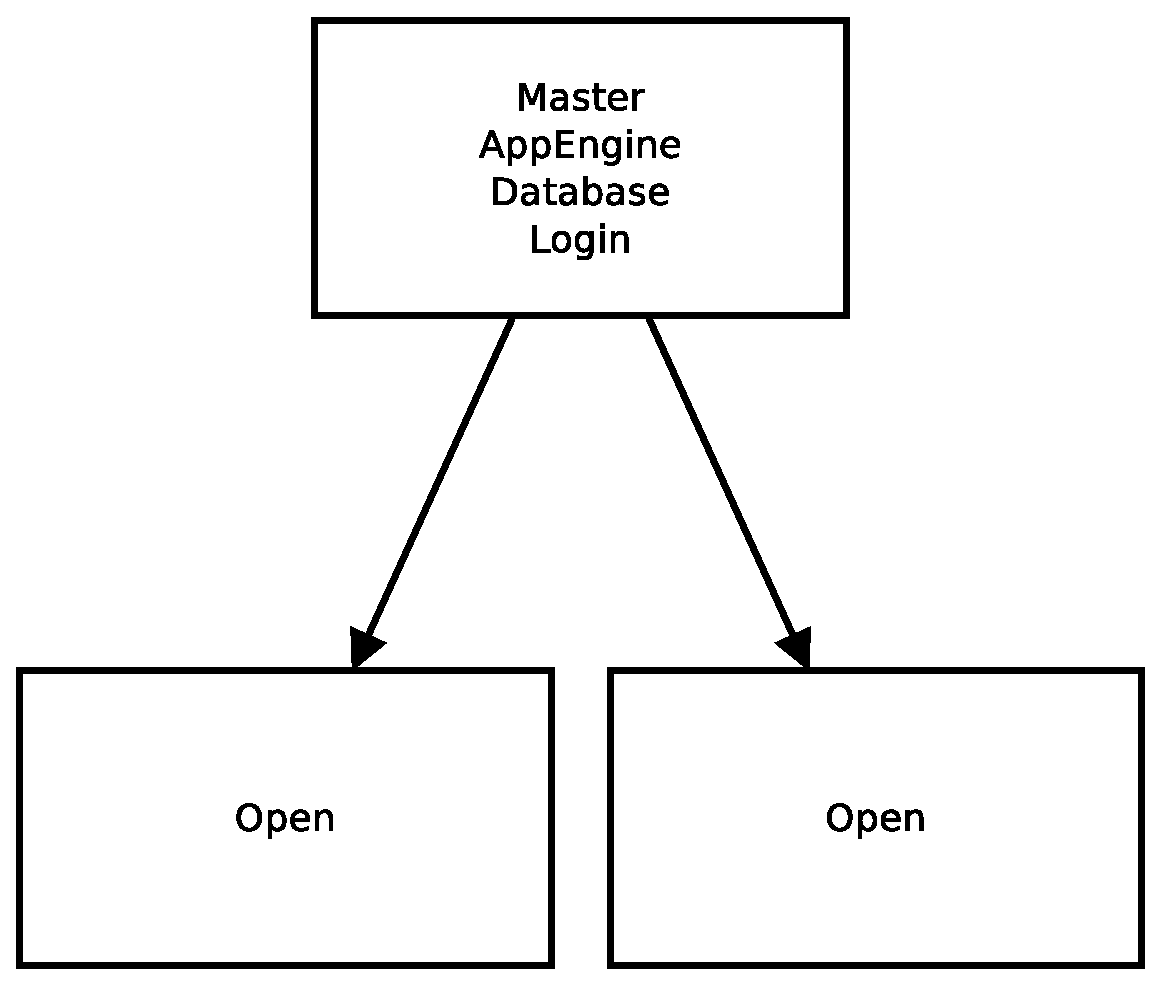
\includegraphics[width=0.5\textwidth]{figuras/Arquitectura_AppScale.eps}
  \caption{Infraestructura AppScale en despliegue personalizado.}
\label{figure:arquitectura-appscale}
\end{figure}

Además de los atributos necesarios para los roles de las máquinas, el tipo \texttt{appscale} también debe contar con la cuenta de correo y la contraseña para el administrador del \emph{cloud}. Los atributos más importantes del tipo \texttt{appscale} (ver Anexo X para implementación completa), en lo que a ejecución de trabajos concierne, son:

\begin{rubycode}
Puppet::Type.newtype(:appscale) do
   @doc = "Manages AppScale clouds formed by KVM virtual machines."
   
   # ...

   # AppScale parameters
   
   newproperty(:master, :array_matching => :all) do
      desc "The master node"
   end

   newproperty(:appengine, :array_matching => :all) do
      desc "The appengine nodes"
   end

   newproperty(:database, :array_matching => :all) do
      desc "The database nodes"
   end

   newproperty(:login, :array_matching => :all) do
      desc "The login node"
   end

   newproperty(:open, :array_matching => :all) do
      desc "The open nodes"
   end
   

   newparam(:app_email) do
      desc "AppScale administrator e-mail"
      defaultto "david@gmail.com"
   end
   
   newparam(:app_password) do
      desc "AppScale administrator password"
      defaultto "appscale"
   end

end
\end{rubycode}

Para lograr un despliegue de este tipo podría utilizarse un manifiesto similar a éste:

\begin{lstlisting}
appscale {'mycloud':
   master    => ["155.210.155.73",
                 "/var/tmp/dceresuela/lucid-tor1.img"],
   appengine => ["155.210.155.73",
                 "/var/tmp/dceresuela/lucid-tor1.img"],
   database  => ["155.210.155.73",
                 "/var/tmp/dceresuela/lucid-tor1.img"],
   login     => ["155.210.155.73",
                 "/var/tmp/dceresuela/lucid-tor1.img"],
   open      => ["/etc/puppet/modules/appscale/files/open-ips.txt",
                 "/etc/puppet/modules/appscale/files/open-imgs.txt"],
   vm_domain => "/etc/puppet/modules/appscale/files/mycloud-template.xml",
   pool => ["155.210.155.70"],
   ensure => running,
}
\end{lstlisting}


%%%%%%%%%%%%%%%%%%%%%%%%%%%%%%%%%%%%%%%%%%%%%%%%%%%%%%%%%%%%%%%%%%%%%%%%%%%%%%%%
\section{Diseño e implementación de un recurso distribuido para una infraestructura TORQUE}

Una infraestructura TORQUE está formada por un nodo maestro y un conjunto de nodos de computación (Figura \ref{figure:arquitectura-torque}). El nodo maestro es el encargado de recibir los trabajos a ejecutar y de asegurar una correcta planificación para esos trabajos; en su versión más simple el planificador es una cola FIFO. Los nodos de computación son los encargados de ejecutar los trabajos enviados por el nodo maestro y, una vez terminados, enviarle los resultados de vuelta. \\

\begin{figure} [!htbp]
  \centering
  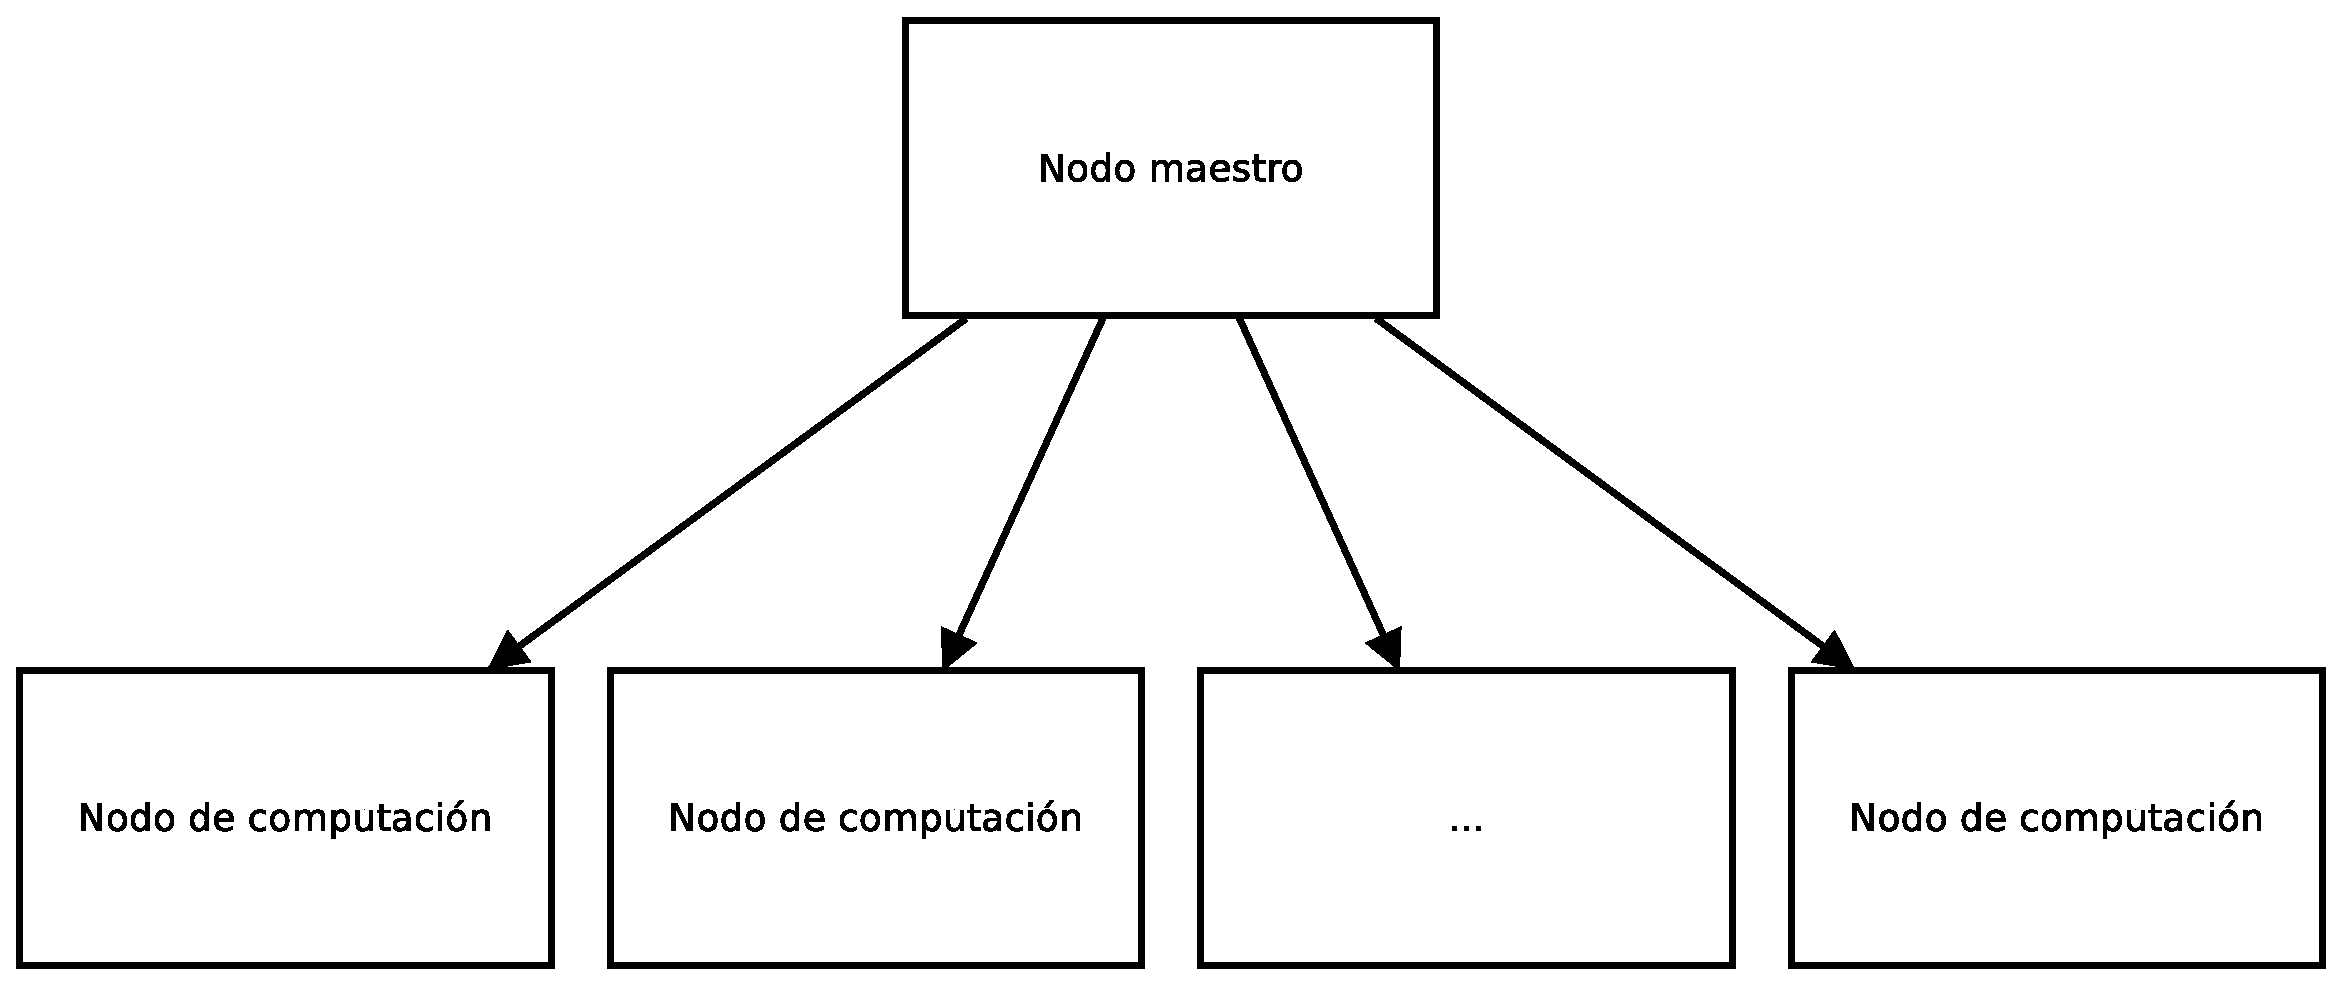
\includegraphics[width=13.5cm]{figuras/Arquitectura_Torque.eps}
  \caption{Infraestructura Torque.}
\label{figure:arquitectura-torque}
\end{figure}

Los nuevos atributos que aparecen en el tipo \texttt{torque} reflejan esta nueva infraestructura:

\begin{rubycode}
Puppet::Type.newtype(:torque) do
   @doc = "Manages Torque clouds formed by KVM virtual machines."
   
   # ...

   # Torque parameters
   newproperty(:head, :array_matching => :all) do
      desc "The head node's information"
   end
   
   newproperty(:compute, :array_matching => :all) do
      desc "The compute nodes' information"
   end
   
end
\end{rubycode}

La sintaxis del manifiesto de puesta en marcha también se modifica para reflejar este cambio. Un ejemplo de un manifiesto para la puesta en marcha de una infraestructura TORQUE sería similar a éste:

\begin{lstlisting}
torque {'mycloud':
   head => ["155.210.155.73", "/var/tmp/dceresuela/lucid-tor1.img"],
   compute => ["/etc/puppet/modules/torque/files/compute-ips.txt",
               "/etc/puppet/modules/torque/files/compute-imgs.txt"],
   vm_domain => "/etc/puppet/modules/torque/files/mycloud-template.xml",
   pool => ["155.210.155.70"],
   ensure => running,
}
\end{lstlisting}

%Por otro lado, un posible manifiesto de parada sería similar a éste:

%\begin{lstlisting}
%torque {'mycloud':
%   head => ["155.210.155.73", "/var/tmp/dceresuela/lucid-tor1.img"],
%   compute => ["/etc/puppet/modules/torque/files/compute-ips.txt",
%               "/etc/puppet/modules/torque/files/compute-imgs.txt"],
%   pool => ["155.210.155.70"],
%   ensure => stopped,
%}
%\end{lstlisting}

